\documentclass[10pt, letterpaper]{article}
%\documentclass[10pt,twocolumn,letterpaper]{article}
% \usepackage[a4paper, total={6in, 8in}]{geometry}
\usepackage{cvpr}
\usepackage{times}
\usepackage{epsfig}
\usepackage{graphicx}
\usepackage{amsmath}
\usepackage{amssymb}
\usepackage{enumitem}
\usepackage{url}
\usepackage{mathrsfs}
\usepackage{float}
\usepackage{amsfonts,nicefrac,mathtools,bbm,color}
\usepackage{verbatim}

\newcommand{\real}{\mathbb{R}}

\newcommand{\bsx}{\boldsymbol{x}}

\newcommand{\e}{\mathbb{E}}
\newcommand{\var}{\mathrm{var}}

\newcommand{\rct}{\mathcal{R}}
\newcommand{\odb}{\mathcal{O}}

\newcommand{\err}{\varepsilon}

\renewcommand{\le}{\leqslant}
\renewcommand{\ge}{\geqslant}

\newcommand{\tran}{\mathsf{T}}

\newcommand{\simiid}{\stackrel{\mathrm{iid}}\sim}

\newcommand{\rd}{\,\mathrm d}

% Specialized notation. 
% Small roman subscripts are more readable than smal italic ones.

\renewcommand{\k}{\mathrm{k}}
\renewcommand{\r}{\mathrm{r}}
\newcommand{\s}{\mathrm{s}}
\renewcommand{\o}{\mathrm{o}}

\newcommand{\rk}{\mathrm{rk}}
\newcommand{\rkt}{\mathrm{rkt}}
\newcommand{\rkc}{\mathrm{rkc}}
\newcommand{\rt}{\mathrm{rt}}
\newcommand{\rc}{\mathrm{rc}}

\newcommand{\ok}{\mathrm{ok}}
\newcommand{\okt}{\mathrm{okt}}
\newcommand{\okc}{\mathrm{okc}}

\newcommand{\ot}{\mathrm{ot}}
\newcommand{\oc}{\mathrm{oc}}

\newcommand{\sk}{\mathrm{sk}}
\newcommand{\skt}{\mathrm{skt}}
\newcommand{\skc}{\mathrm{skc}}

\newcommand{\st}{\mathrm{st}}
\renewcommand{\sc}{\mathrm{sc}}


\newcommand{\nr}{n_{\r}}
\newcommand{\nrk}{n_{\rk}}
\newcommand{\nrkt}{n_{\rkt}}
\newcommand{\nrkc}{n_{\rkc}}

\newcommand{\nrt}{n_{\rt}}
\newcommand{\nrc}{n_{\rc}}


\newcommand{\no}{n_{\o}}
\newcommand{\nok}{n_{\ok}}
\newcommand{\nokt}{n_{\okt}}
\newcommand{\nokc}{n_{\okc}}

\newcommand{\fr}{f_{\r}}
\newcommand{\fo}{f_{\o}}

\newcommand{\byr}{\bar Y_{\r}}
\newcommand{\byrk}{\bar Y_{\rk}}
\newcommand{\byrkt}{\bar Y_{\rkt}}
\newcommand{\byrkc}{\bar Y_{\rkc}}

\newcommand{\byrt}{\bar Y_{\rt}}
\newcommand{\byrc}{\bar Y_{\rc}}

\newcommand{\byo}{\bar Y_{\o}}
\newcommand{\byok}{\bar Y_{\ok}}
\newcommand{\byokt}{\bar Y_{\okt}}
\newcommand{\byokc}{\bar Y_{\okc}}

% Include other packages here, before hyperref.

% If you comment hyperref and then uncomment it, you should delete
% egpaper.aux before re-running latex.  (Or just hit 'q' on the first latex
% run, let it finish, and you should be clear).
\usepackage[breaklinks=true,bookmarks=false]{hyperref}

\cvprfinalcopy % *** Uncomment this line for the final submission

\def\httilde{\mbox{\tt\raisebox{-.5ex}{\symbol{126}}}}

% Pages are numbered in submission mode, and unnumbered in camera-ready
%\ifcvprfinal\pagestyle{empty}\fi
\setcounter{page}{1}
\begin{document}

%%%%%%%%% TITLE
\title{Using Poisson Binomial GLMs to Model Voter Behavior}

\author{Evan Rosenman\\
Stanford University\\
{\tt\small rosenman@stanford.edu}
% For a paper whose authors are all at the same institution,
% omit the following lines up until the closing ``}''.
% Additional authors and addresses can be added with ``\and'',
% just like the second author.
% To save space, use either the email address or home page, not both
\and
Nitin Viswanathan\\
Stanford University\\
{\tt\small nviswana@stanford.edu}
}

\maketitle
%\thispagestyle{empty}

%%%%%%%%% ABSTRACT
% \begin{abstract}
% TODO
% \end{abstract}

%%%%%%%%% BODY TEXT
\section{Introduction}
Political organizations seek to build voting models to explain voter preferences, as this information is vital for voter targeting. In the US, voting data indicating how many votes every candidate receives is available at the precinct level, but the most granular data – who voted for which candidate – is private. As a result, political groups are forced to rely on polling data to perform analysis at the individual voter level. Polling data can not only be unreliable but it is also incomplete, as voters are not obligated to express their true preferences and the majority of voters will not participate in polls. We develop individual voter models based off of publicly available aggregated voting data.

We use precinct-level data across several counties in Pennsylvania from the 2016 presidential election together with individual-level demographic data to model who a given voter will vote for. We focus on predicting votes for both Hillary Clinton and Donald Trump in the state of Pennsylvania as it was a key swing state that went in favor of Donald Trump in the 2016 presidential election. Trump's margin of victory was very slim at only 44,292 votes, only 0.72\% more than Clinton's\cite{NYT}. Precinct-level election results are the most granular results available; for reference there are about 9,000 precincts total in Pennsylvania \cite{NYT}. 

We formulate the problem using a Poisson binomial generalized linear model and maximize the log-likelihood, which has not, to our knowledge, been done before in other literature.

Our paper makes two key contributions:
\begin{itemize}[noitemsep]
	\item We develop the math necessary to use and train Poisson binomial GLMs
	\item We apply poission binomial GLMs to the specific task of predicting voter behavior
\end{itemize}

% taking this out for now, since this is just the milestone
\begin{comment}
More generally, we believe that our development of the Poisson binomial GLMs will be applicable to other problems where the goal is also to build a model explaining individual behavior given aggregate-level performance and individual-level features. Our work can be extended to support Poisson multionomial GLMs as well to model problems where individuals have more than two choices that are then aggregated.
\end{comment}

\section{Dataset}

\subsection{Overview}

We have collected two relevant datasets for our project that we combined together.

Our dataset of \textbf{Pennsylvania precinct-level election results} contains the total number of votes received by each candidate in the 2016 presidential election. We obtained this dataset from OpenElections\cite{OpenElections}.

The second is the \textbf{Pennsylvania voter dataset} which we obtained directly from the Pennsylvania Department of State\cite{PAVoterFile}. This dataset contains a row for every registered voter in Pennsylvania as well as their party registration, limited demographic information (age, gender), and voting participation over a set of recent primaries and general elections.

For the milestone, we focused on four of Pennsylvania's 67 counties: Adams, Allegheny, Bedford, and Chester. These counties are diverse -- Allegheny and Chester were won by Clinton while Adams and Bedford were won by Trump. Together they represent 1,639 precincts and about 950,000 total votes for Clinton and Trump. 

\subsection{Dataset Preparation and Validation}

Because these files were sourced from two different datasets, we ran into some challenges in cleanly mapping them with each other. We had to match precincts between the two files based on name instead of some sort of unique code or identifier. After our initial checks these worked fine for the four counties we selected for the milestone, and one of our next steps will be to investigate this further and get a mapping across all precincts and counties in Pennsylvania to have more usable data. 

We only model based on the vote counts for Hillary Clinton and Donald Trump because the vast majority of votes cast were for one of them. Our datasets are not perfectly accurate because some voters voted for candidates besides Clinton and Trump and also because voters can fill out a ballot but not select a presidential candidate, voting only in other races (e.g. local ones) instead. Upon examining our dataset we noticed that the sum of Clinton/Trump votes in precincts is not equal to the total number of votes cast in the precinct, but is within 10\% in most cases. To address these data issues, we take the percentage of Clinton/Trump votes cast in a precinct went to Clinton and multiply it by the total number of Clinton/Trump votes in the precinct, and repeat this for Trump. This number is our estimate of how many voters in a precinct would have went for Clinton/Trump if these two candidates were the only two options.

\section{Methods}

\subsection{Poisson Binomial GLM form}

We use a Generalized Linear Model based on the Poisson binomial distribution. We model an individual $i$ voting for Clinton as a Bernoulli random variable, so $p_i = \sigma(\theta^TX_i)$, where $\sigma(.)$ denotes the sigmoid function, $\theta$ is a set of parameters to fit, and $X_i$ are known covariates from the Pennsylvania voter dataset. Note that the probability of an individual voting not voting for Clinton (i.e. voting for Trump) is $1 - p_i$. We assume that these Bernoulli random variables are independent but not necessarily identically distributed, since we expect that different voters would have different probabilities of voting for Clinton.

Combining this representation of a voter with the fact that in a given precinct we know the total number of votes for Clinton and Trump, the total number of Clinton voters in each precinct will follow a Poisson binomial distribution, which is the probability distribution of a sum of independent but not necessarily identically distributed Bernoulli random variables\cite{Poibi}. For a precinct $k$ with $D$ votes for Clinton out of $T$ total votes, the likelihood is given by:

$$\ell_k(\theta) = \sum_{A \in F_k} \prod_{i \in A} p_i \prod_{j \in A^c}(1 - p_j)$$
where $F_k$ is the set of all configurations of $T$ votes in which a total of $D$ votes were cast for Clinton; $A$ is the set of voters who voted for Clinton under that configuration, and $A^c$ is the set of voters who voted for Trump under that configuration. The likelihood of the precinct-level results given parameters $\theta$ can be calculated by multiplying the likelihoods from every precinct together:

$$\ell(\theta) = \prod_k \ell_k(\theta)$$

In order to determine the optimal parameters $\theta$, we need to maximize this likelihood over the Pennsylvania precincts. Note that the Poisson binomial likelihood involves sums over all possible configurations of votes -- e.g. if Clinton received 200 out of 500 total votes in a precinct, then the likelihood involves a sum over $500 \choose 200$ configurations. Although we can directly estimate the likelihood well using discrete Fourier transforms (as the \texttt{poibin} package does\cite{PoibiGithub}), computing the gradient is computationally intractable.

\subsection{Calculating the Gradient}

To address this problem, we make use of the Lyapunov CLT\cite{LyapunovCondition} to observe that the asymptotic distribution of $d_k$, the number of votes for Clinton in precinct $k$, is given by: 
\[ d_k \stackrel{d} \longrightarrow N \left(\sum_{i} p_{k,i}, \sum_{i} p_{k, i}(1-p_{k, i}) \right) \] 
where $p_{k, i}$ is the $i^{th}$ entry of $p_k$. This result is proven in the appendix. It allows us to \emph{estimate} the likelihood with a much simpler function of $\theta$. In this case, the contribution of precinct $k$ to the overall log-likelihood is approximately: 
\[ \ell_k = -log \left( \phi_k\right) + \frac{1}{\phi_k^2} \left( d_k -\mu_k \right)^2  \] 
where irrelevant constants have been dropped, $\mu_k =  \sum_{i} p_{k, i}(1-p_{k, i}), \phi_k^2 = \sum_{i} p_{k, i}(1-p_{k, i})$, and $p_{k, i} = \sigma(\theta^T x_{k, i})$. This yields a gradient of the form: 
\begin{align*}
\nabla_{\theta} \ell_k &=  \frac{1}{2} \left(\frac{(d_k - \mu_k)^2}{\phi^4} - \frac{1}{\phi^2} \right) \left( \sum_{i} (2 p_{k, i} - 1)p_{k, i}^2 x_{k, i} \right) + \frac{1}{\phi^2} (d_k - \mu_k) \left( \sum_i p_{k, i} (1 - p_{k, i}) x_{k, i} \right)
\end{align*}

% \section{Experiments}

% \subsection{Setup}

% \subsection{Implementation Details}
% we used stochastic gradient descent, iterating over precincts. went one at a time instead of batch/minibatch since precincts are large. maybe it's worth doing batch?
% Hyperparameters, regularization, optimization methods etc. go here

% \subsection{Evaluation Metrics}

\section{Preliminary Results}

Using stochastic gradient ascent, we fit a simple model to the four counties where we predict the probability to vote for Clinton given county, party registration, primary participation, gender, and age. Computing the log-likelihood every 25 iterations, we see a modest improvement over the first 400 iterations (after which the log-likelihood plateaus): 
\begin{figure}[H]
\centering
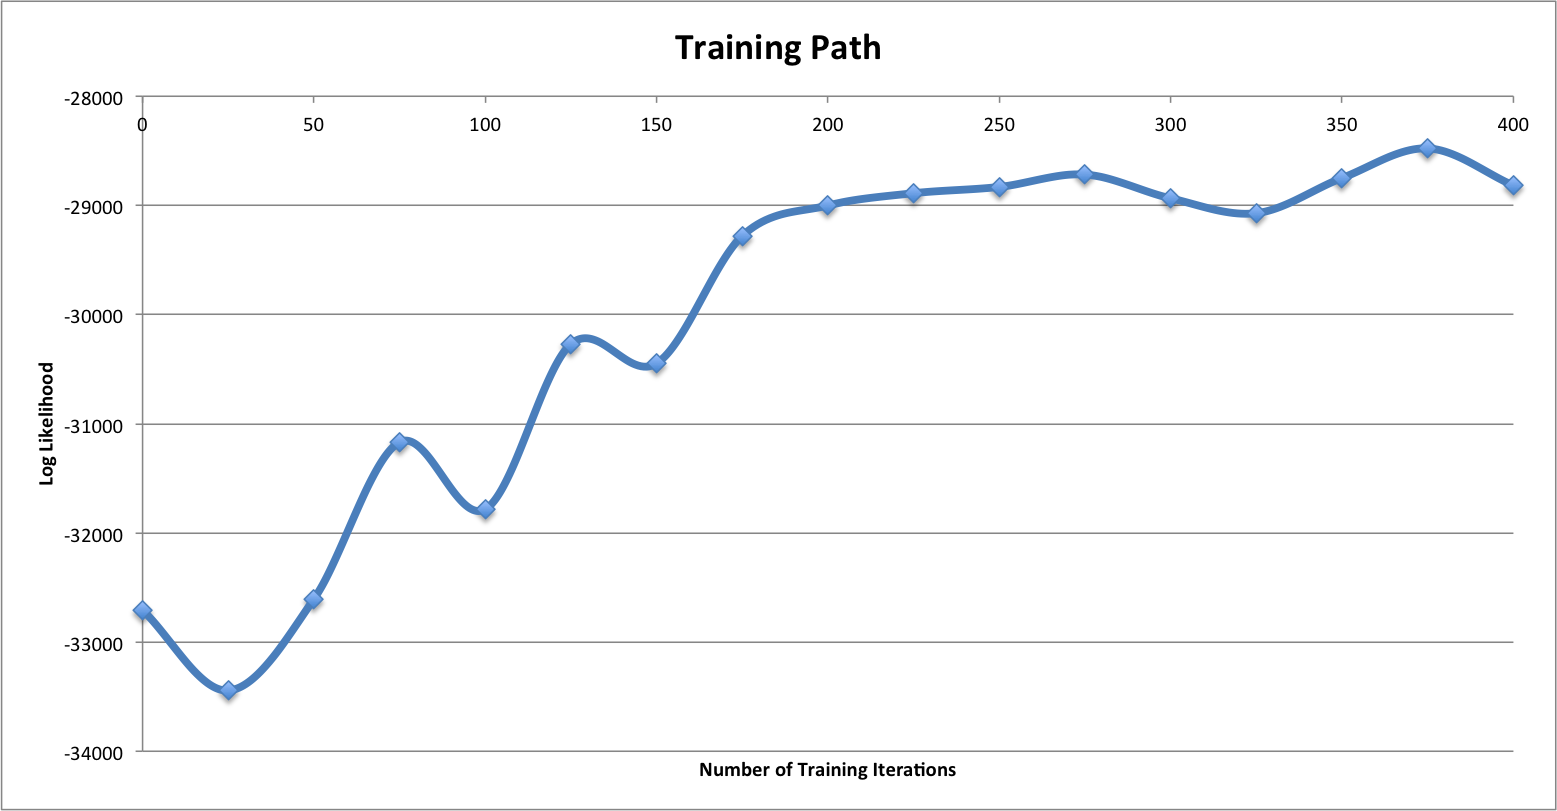
\includegraphics[scale = 0.4]{TrainingPath}
\end{figure}

Below we present the coefficients coming out of the model, noting that positive values indicate that a voter is more likely to vote for Clinton over Trump:

\begin{table}[H]
\centering
\begin{tabular}{|l|l|l|l|l|lll}
\cline{1-2} \cline{4-5} \cline{7-8}
is Chester resident?   & 0.61  &  & is registered Democrat?      & 0.30  & \multicolumn{1}{l|}{} & \multicolumn{1}{l|}{is Female?} & \multicolumn{1}{l|}{0.03}  \\ \cline{1-2} \cline{4-5} \cline{7-8} 
is Adams resident?     & -0.42 &  & is registered Republican?    & -0.52 & \multicolumn{1}{l|}{} & \multicolumn{1}{l|}{is Male?}   & \multicolumn{1}{l|}{-0.05} \\ \cline{1-2} \cline{4-5} \cline{7-8} 
is Bedford resident?   & -0.78 &  & voted in Democratic primary? & 0.18  & \multicolumn{1}{l|}{} & \multicolumn{1}{l|}{Age}        & \multicolumn{1}{l|}{-0.26} \\ \cline{1-2} \cline{4-5} \cline{7-8} 
is Allgeheny resident? & 0.39  &  & voted in Republican primary? & -0.30 &                       &                                 &                            \\ \cline{1-2} \cline{4-5}
\end{tabular}
\end{table}
These results are in line with what we would expect. For example, older voters are more likely to vote for Trump and registered Democrats are more likely to vote for Clinton.

\section{Next Steps}

Our initial results are encouraging. Our main next step is to run our model with more data, using as much of Pennsylvania as we can use. We would also like to fit more complex models with more predictors, possibly incorporating data from sources beyond the Pennsylvania voter file itself such as demographics if we can obtain them. As we obtain more data and fit more complex models, it will be important to make sure that we are converging efficiently. We are currently performing vanilla stochastic gradient descent, and we will investigate other optimization techniques such as Adam.

Once we are able to train on more data, we will split our data into training and test sets instead of training on all of it. Our plan is to train our model on 70\% of the precincts in Pennsylvania and then test on the remaining 30\% to gauge model accuracy, using the total number of Clinton and Trump votes per precinct as the outcome variable. We are are particularly curious to see if our approach (modeling at the individual level) can yield better predictions than modeling at the precinct level by aggregated individual-level features. There are many approaches to modeling at the precinct level (e.g. linear regression, neural nets) that we can compare against. We will also see if we can compare our approach against existing voter models that use polling data.

Once we begin training our model on only a training set and evaluating it on a holdout, we will experiment with adding regularization to see if it improves performance. In addition to gradient descent, we would also like to explore alternative methods for maximizing the log likelihood such as numerical gradients and expectation maximization.

\section{Contributions}
Evan and Nitin both worked together to define the problem and scope it out as a Poisson GLM, and find the Pennsylvania state and OpenElections datasets. Evan wrote the majority of code for the progress made so far for the milestone and derived the CLT proof, while Nitin wrote up the milestone report as well as additional sections that will be useful for the final project report and focused on establishing better data mappings between our two datasets.


\newpage
\section*{Appendix: Lyapunov CLT Proof}

Define $d_k = \sum_{i = 1}^n d_{k, i}$ to be the number of Democratic votes in precinct $k$, where $d_{k, i}$ is an indicator variable denoting whether person $i$ in precinct $k$ voted for Clinton. We know that $d_k$ follows a Poisson binomial distribution with success probabilities $p_k = (p_{k, 1}, \dots, p_{k, n})$. Define:
\[ s_{k}^2 = \sum_{i = 1}^{n} p_{k, i} (1-p_{k, i}) \] 
We check the Lyapunov CLT condition for the fourth moment of the Bernoulli distribution\cite{BernoulliDist}: 
\begin{align*}
\lim_{n \to \infty} \frac{1}{s_k^4} \sum_{i = 1}^n E \left( (d_{k, i} - p_{k, i})^4 \right) &= \lim_{n \to \infty} \frac{\sum_{i = 1}^n p_{k, i}(1-p_{k, i}) \left( 3p_{k, i}^2 - 3p_{k, i} + 1 \right)}{\left(\sum_{i = 1}^n p_{k, i} \left( 1- p_{k, i} \right) \right)^2} \stackrel{?} = 0 
\end{align*}

Observe that $3p_{k, i}^2 - 3p_{k, i} + 1 \in (0, 1)$ if $p_{k, i} \in (0, 1)$. Hence, the numerator is strictly less than $\sum_{i = 1}^n p_{k, i} (1 - p_{k, i})$. Hence, if we can guarantee the numerator grows without bound, then this limit is 0 and the Lyapunov CLT applies. We can do so using a simple condition, like enforcing that there is some $\epsilon > 0$ such that $\epsilon < \bar p_i < 1- \epsilon$ for all $i$ (i.e. the mean probability of voting for Clinton in a precinct never falls below some low threshold $\epsilon$ or above some high threshold $1-\epsilon$). 

The Lypaunov CLT now tells us that: 
\[ \frac{d_k - \sum_{i = 1}^{n} p_{k, i} }{s_k} \stackrel{d} \longrightarrow N(0, 1) \] 
giving us the desired asymptotic normality. 

{\small
\bibliographystyle{ieee}
\bibliography{csbib}
}


\end{document}
